\section{User Difference Analysis}









\subsection{Divergence Metrics}

To characterize differences in commenting behaviour between user groups, we examine two complementary dimensions of divergence:\\ \textbf{content divergence}, which captures differences in the composition of comments, and \textbf{order divergence}, which captures differences in the temporal arrangement of comments within discussions.

\medskip

\noindent\textbf{Content divergence:}
\vspace{0.3cm}
\\
Content divergence measures the extent to which two user groups contribute different sets of comments, independent of their ordering. Given two comment multisets $A$ and $B$, we define this measure using their normalized symmetric difference:
\[
D_{\text{cont}}(A,B)=\frac{|A \triangle B|}{|A|+|B|}.
\]



Lower values indicate greater similarity in the types of comments produced by the two groups, whereas higher values indicate more distinct commenting patterns.



\begin{figure}[!htbp]
\centering
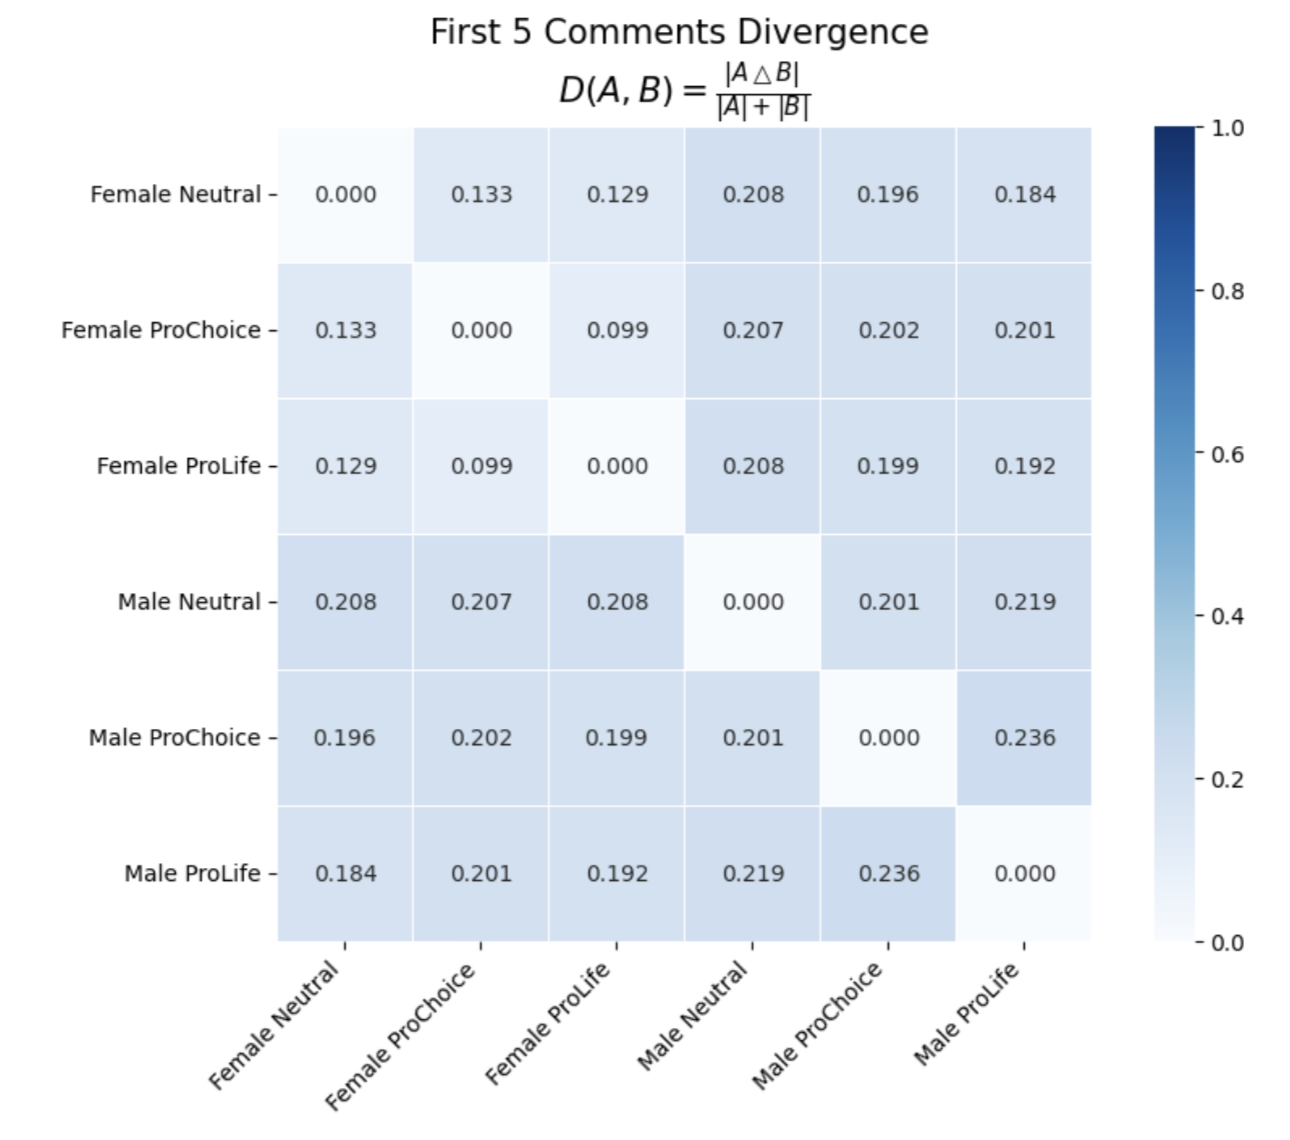
\includegraphics[width=0.65\textwidth]{plots/multiset_divergence_matrix.png}
\caption{Content divergence across user categories based on the first five comments per post.}
\label{fig:multiset_divergence}
\end{figure}

\vspace{1.5cm}

\medskip

\noindent\textbf{Order divergence:}
\vspace{0.5cm}
Beyond differences in comment content, user groups may also differ in how they engage with discussions. Order divergence captures these sequential differences by measuring whether corresponding comments occupy the same positions within discussion threads. For example, which comment appears first, second, and so on.

Formally, given two ordered comment sequences $A$ and $B$ of length $n$, we define:
\[
D_{\text{ord}}(A,B)=\frac{1}{n}\sum_{i=1}^{n}\mathbf{1}_{[A_i \neq B_i]}.
\]
This measure reflects differences in participation dynamics rather than differences in the comments themselves.

\begin{figure}[!htbp]
\centering
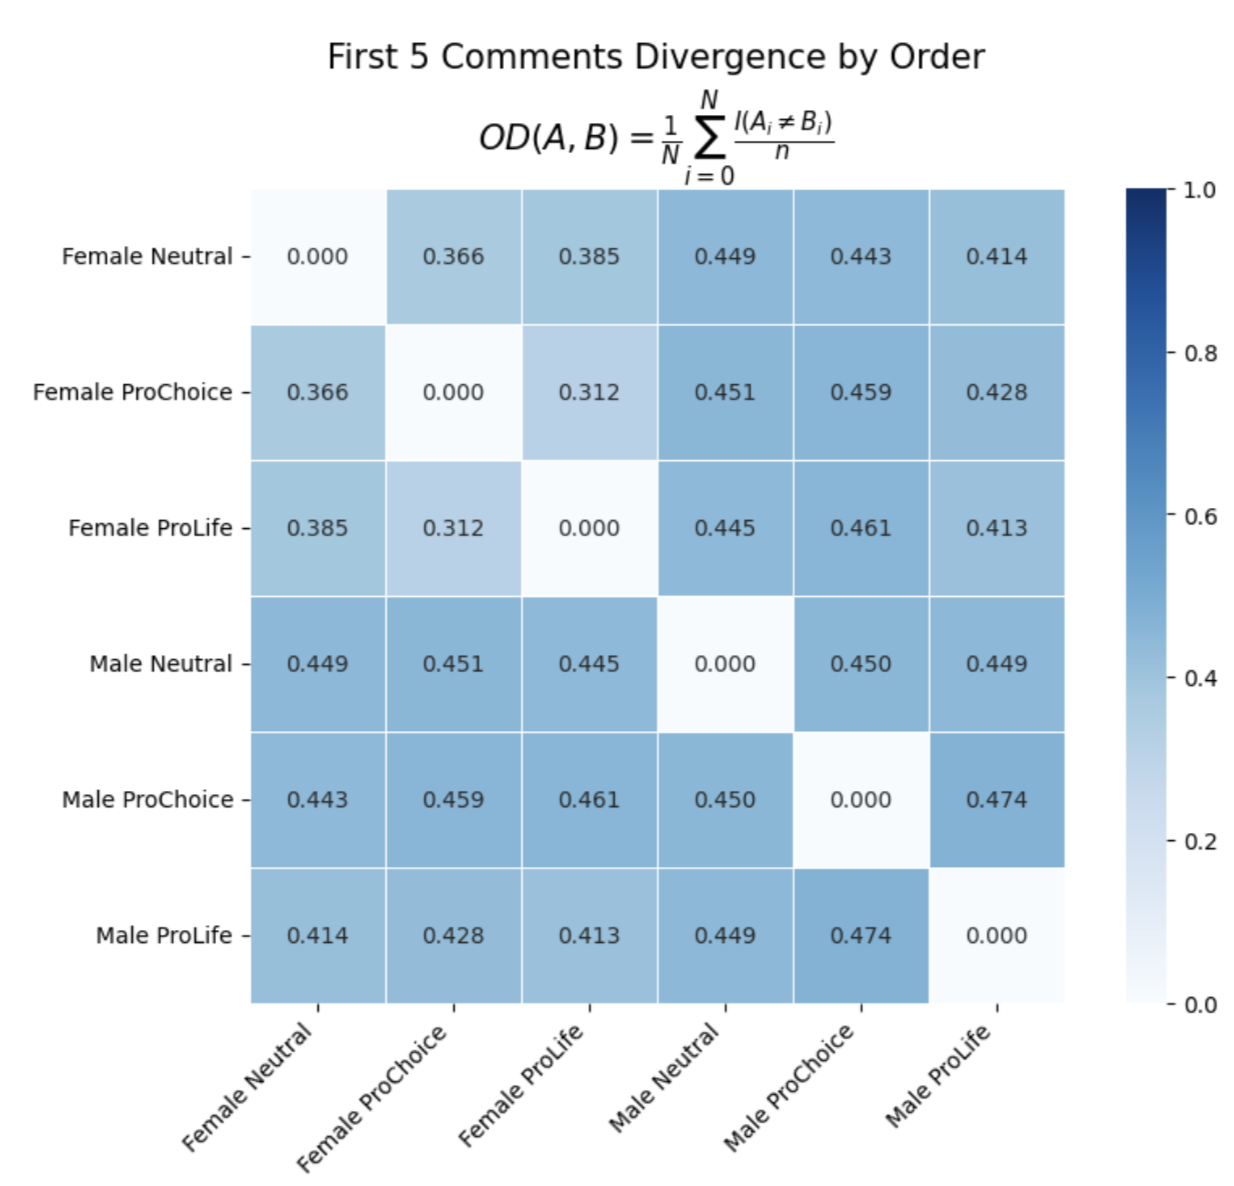
\includegraphics[width=0.65\textwidth]{plots/ordered_divergence_matrix.png}
\caption{Order divergence across user categories based on the first five comments per post.}
\label{fig:ordered_divergence}
\end{figure}
















































\subsection{Comment Depth Effects}

To evaluate how the number of comments considered influences the divergence measures, we progressively increase the comment depth $N$, where $N$ denotes the number of Top comments analysed per post.

\begin{figure}[!htbp]
\centering
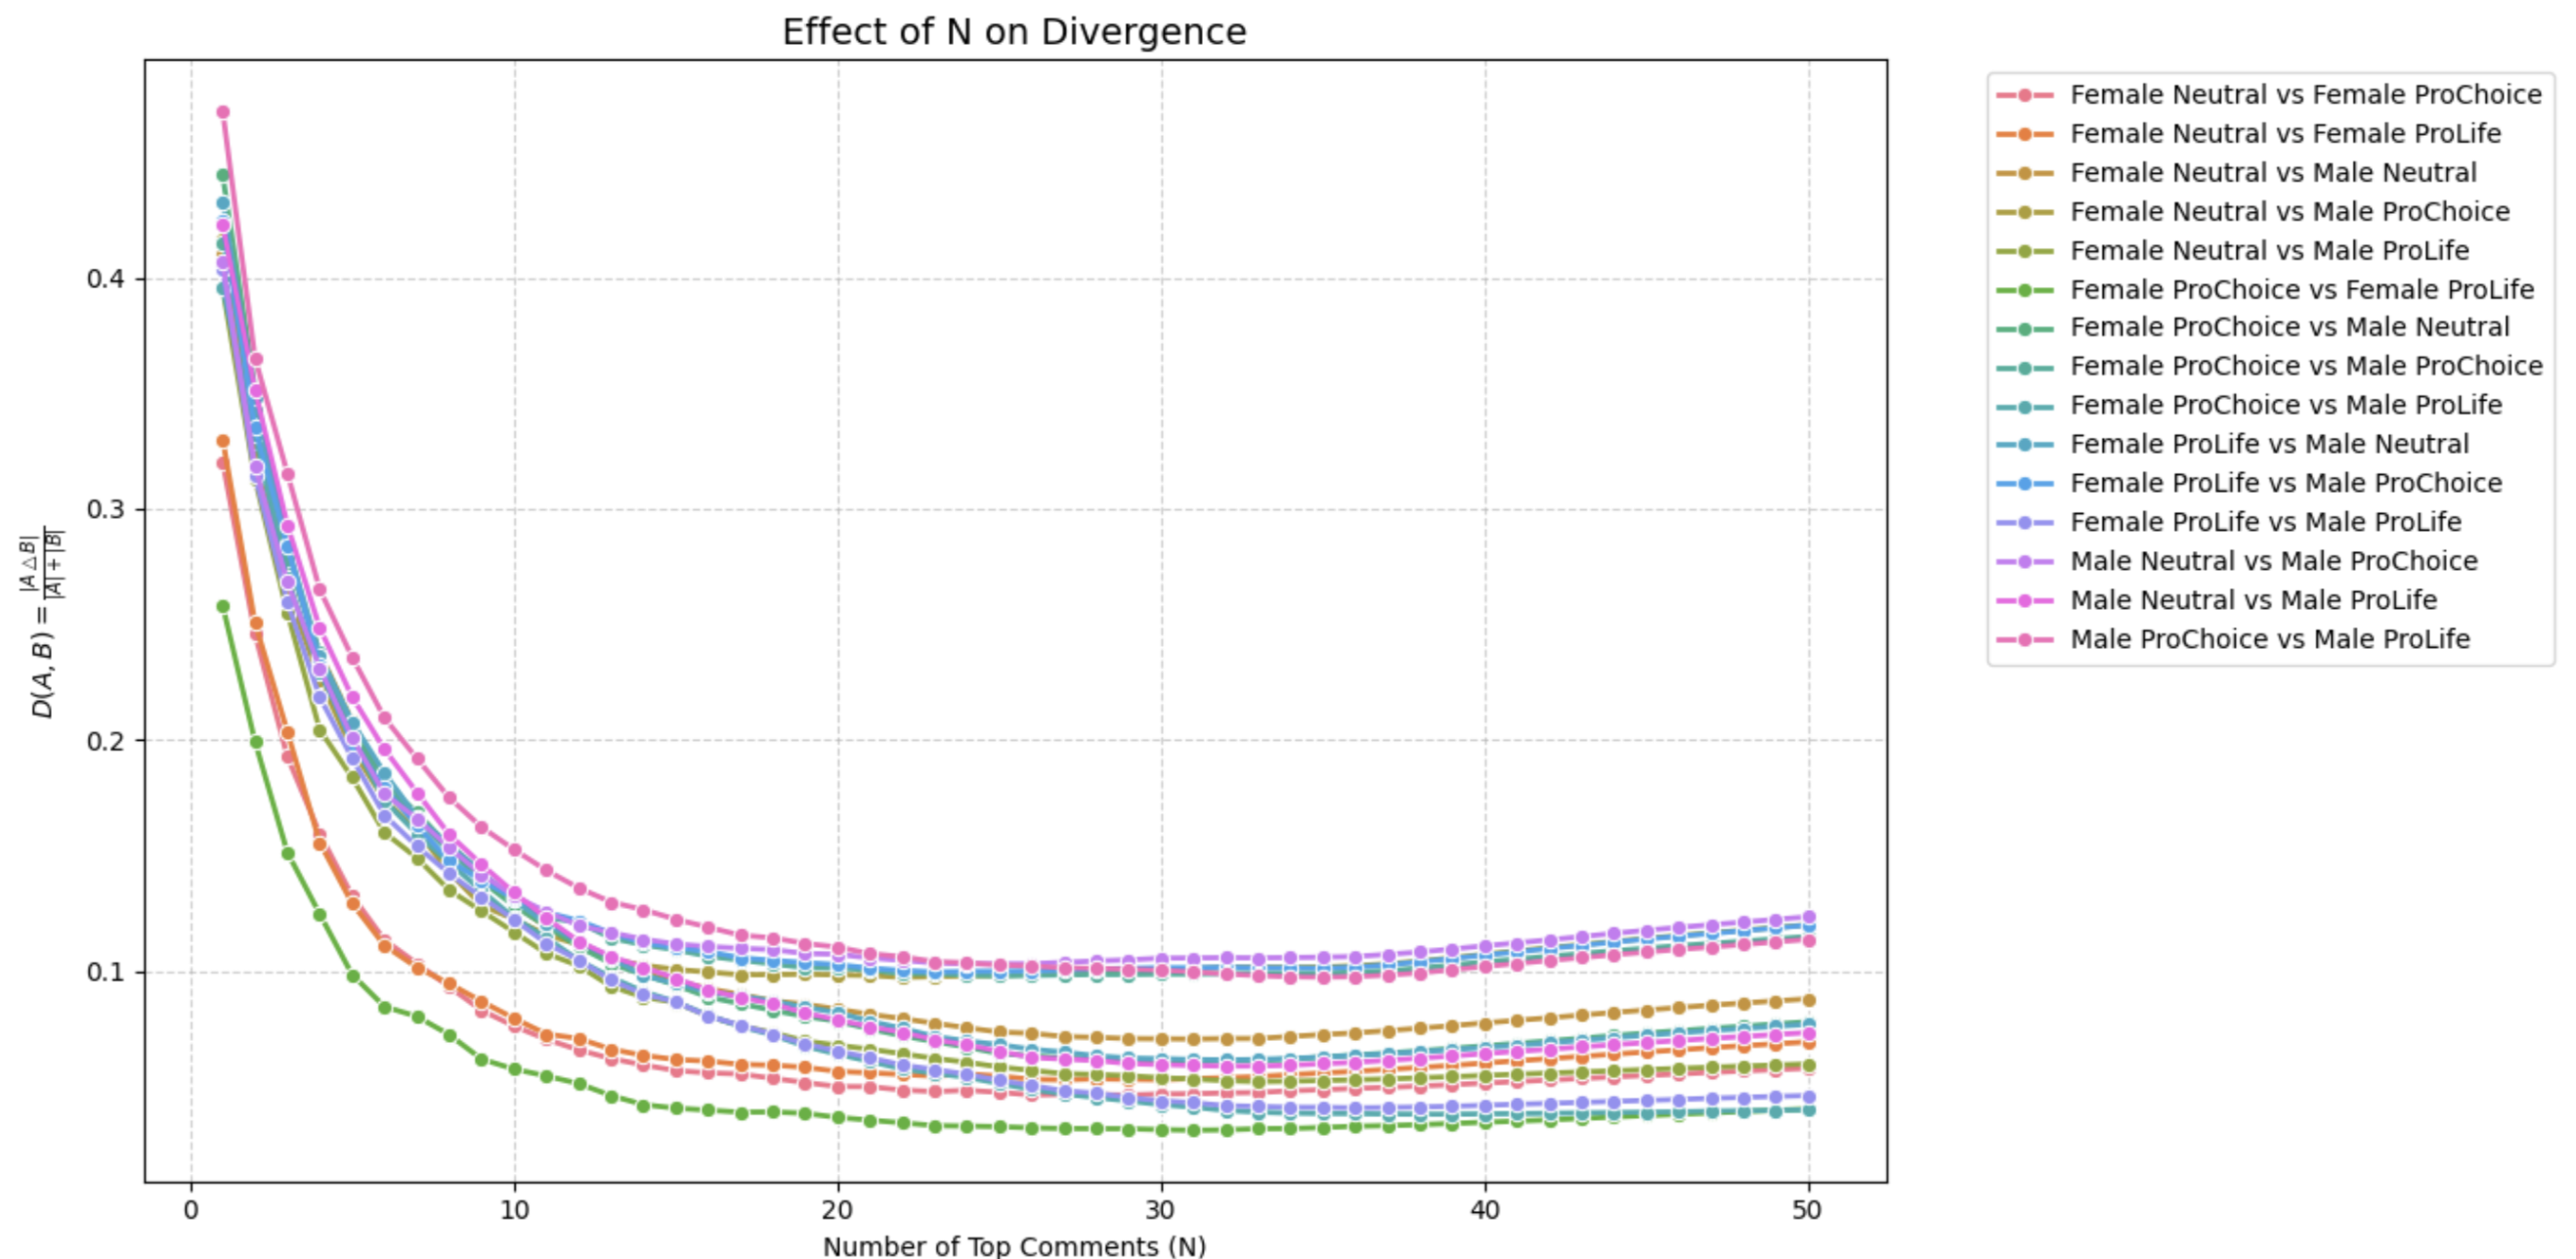
\includegraphics[width=0.75\textwidth]{plots/divergence_vs_n.png}
\caption{Effect of comment depth ($N$) on content divergence.}
\label{fig:divergence_vs_n}
\end{figure}

As shown in Figure~\ref{fig:divergence_vs_n}, content divergence decreases rapidly before converging after approximately 15--20 comments. This suggests that the overall comment composition becomes stable once a sufficient number of comments are included.

\begin{figure}[!htbp]
\centering
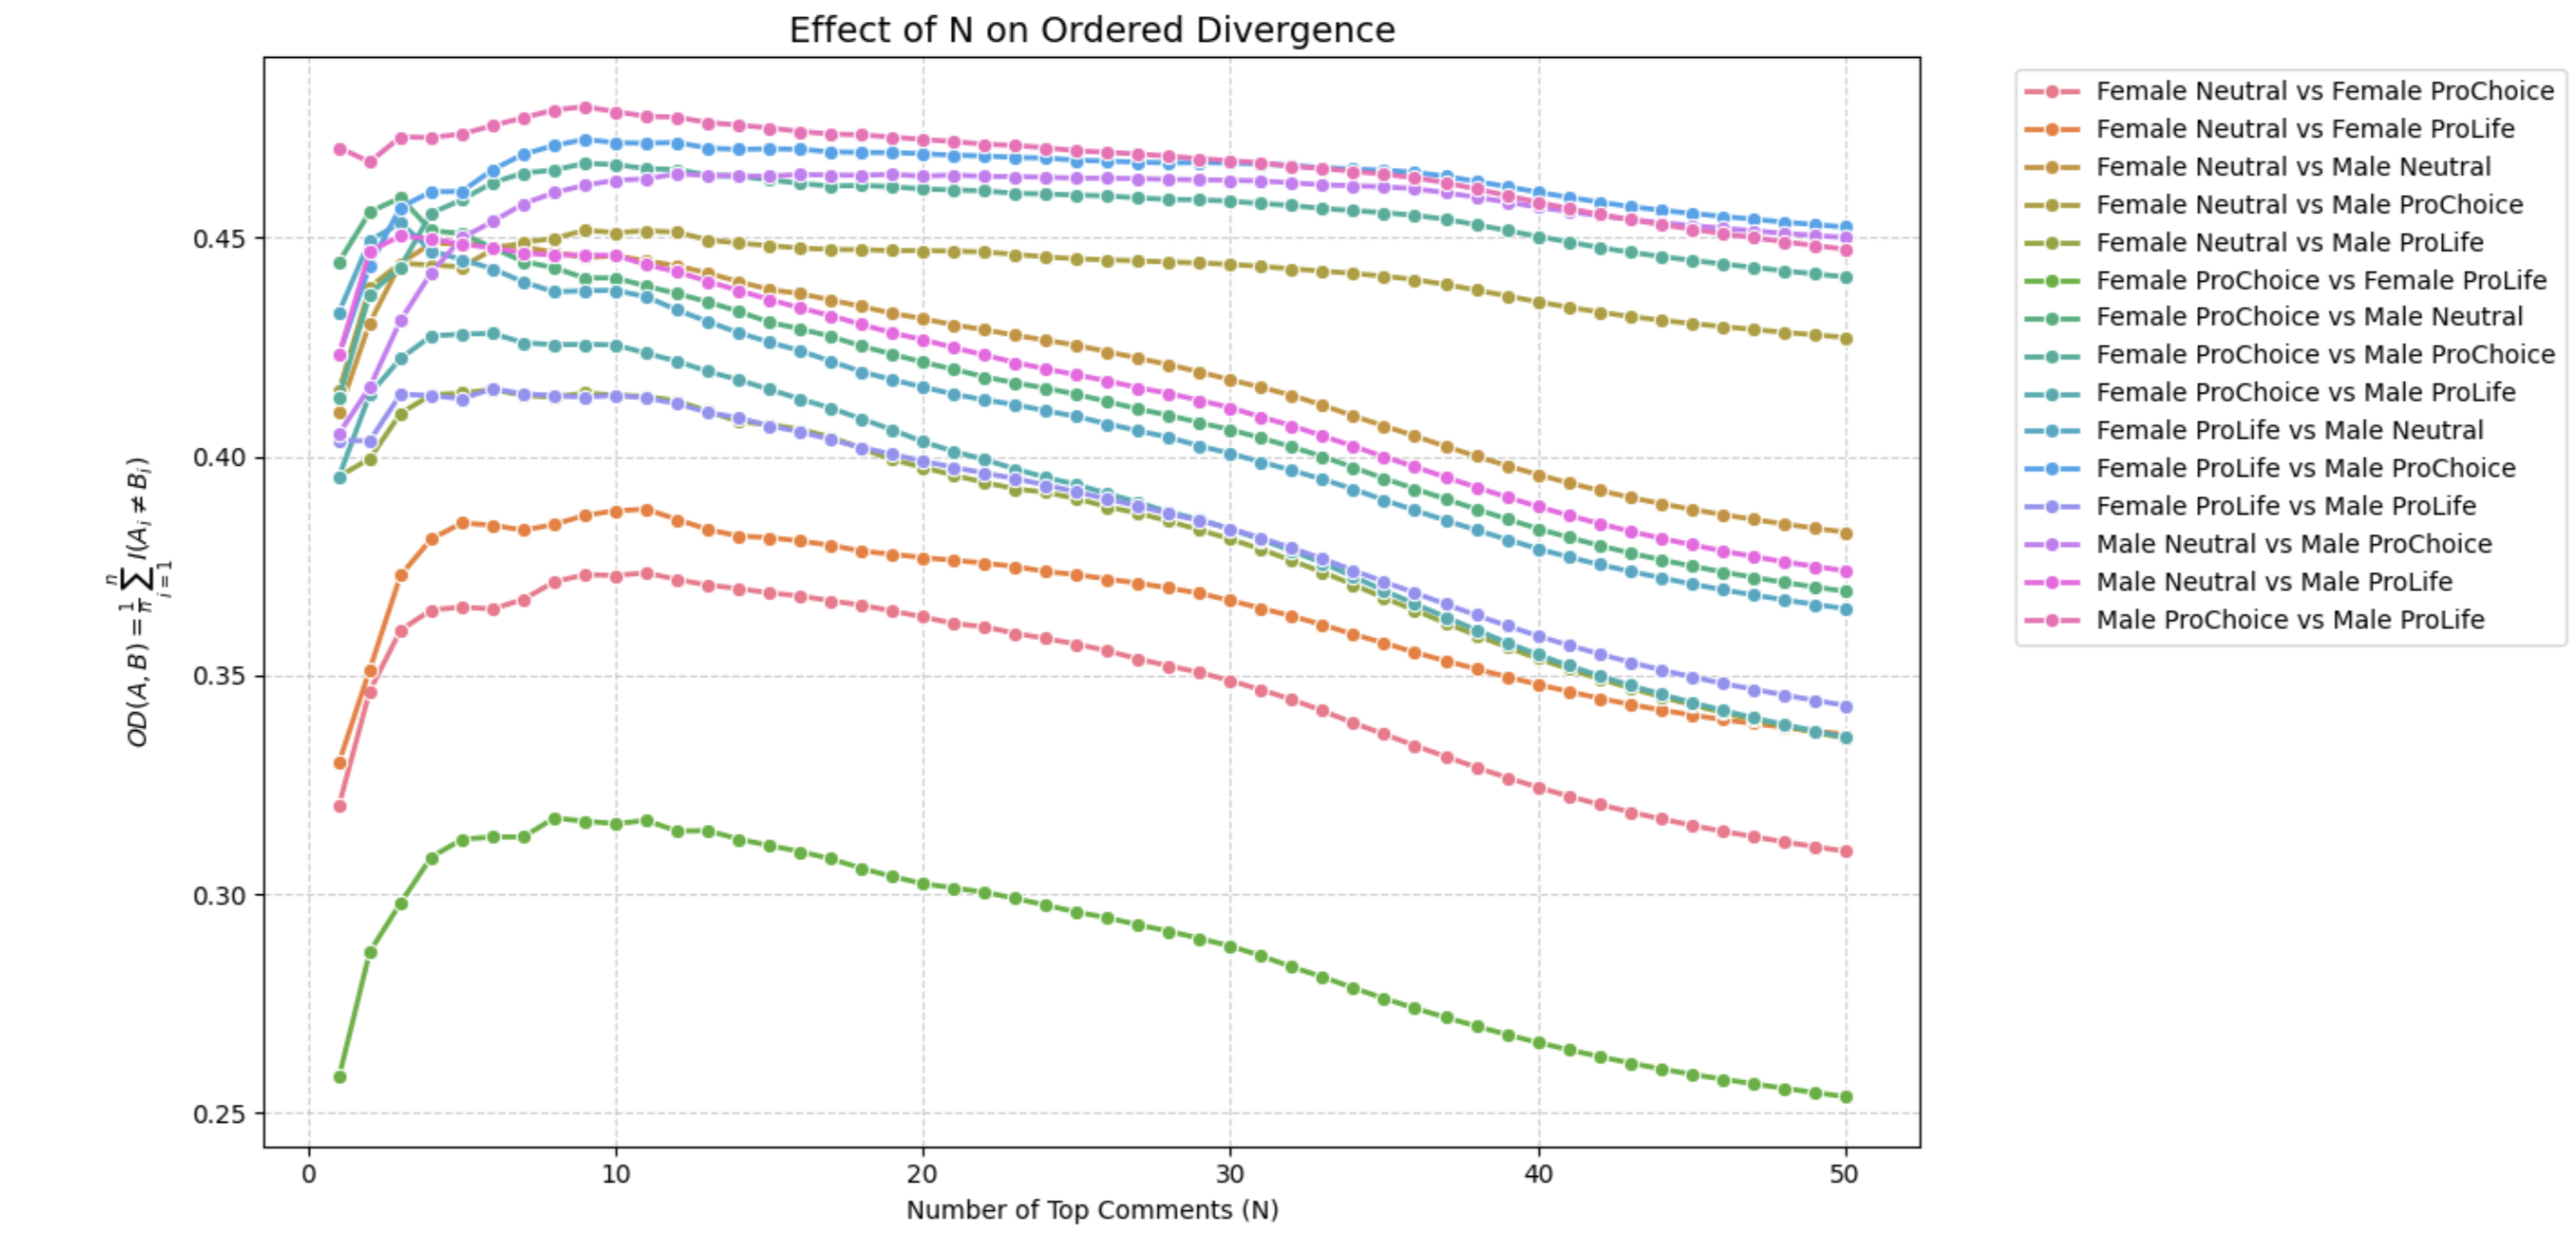
\includegraphics[width=0.75\textwidth]{plots/ordered_divergence_vs_n.png}
\caption{Effect of comment depth ($N$) on ordered divergence.}
\label{fig:ordered_divergence_vs_n}
\end{figure}

In contrast, ordered divergence remains relatively stable across all values of $N$, indicating persistent differences in the temporal ordering of comments. Overall, the results suggest that content differences converge with increasing comment depth, whereas differences in participation dynamics remain consistent throughout the discussion.


\subsection{Discussion}
The divergence analysis shows distinct commenting patterns across user categories. For the first five comments, content divergence is relatively low (0.099--0.236), whereas ordered divergence is considerably higher (0.312--0.474), indicating that differences are more pronounced in participation order than in comment content. The largest divergence is observed between the Male ProChoice and Male ProLife groups, while female groups exhibit the greatest similarity.
These results suggest that commenting behaviour varies across user categories, although the observed differences are likely influenced by additional user- and platform-specific factors beyond gender or stance alone.
